\documentclass[10pt]{article}
\usepackage[utf8]{inputenc}
\usepackage{setspace}
\setstretch{1.2}
\usepackage[T1]{fontenc}
\usepackage{amsmath}
\usepackage{float}
\usepackage{amsfonts}
\usepackage{amssymb}
\usepackage[version=4]{mhchem}
\usepackage{stmaryrd}
\usepackage{graphicx}
\usepackage[export]{adjustbox}
\graphicspath{ {./images/} }
\usepackage{hyperref}
\hypersetup{colorlinks=true, linkcolor=blue, filecolor=magenta, urlcolor=cyan,}
\urlstyle{same}

\title{CM146, Winter 2024 
 Problem Set 1: Decision trees, Nearest neighbors 
 Due Jan 31, 2024 at 11:59 pm PST }

\author{Harris Doan, UID: 605317270}
\date{Winter 2024: Jan 31, 2024}


%New command to display footnote whose markers will always be hidden
\let\svthefootnote\thefootnote
\newcommand\blfootnotetext[1]{%
  \let\thefootnote\relax\footnote{#1}%
  \addtocounter{footnote}{-1}%
  \let\thefootnote\svthefootnote%
}

%Overriding the \footnotetext command to hide the marker if its value is `0`
\let\svfootnotetext\footnotetext
\renewcommand\footnotetext[2][?]{%
  \if\relax#1\relax%
    \ifnum\value{footnote}=0\blfootnotetext{#2}\else\svfootnotetext{#2}\fi%
  \else%
    \if?#1\ifnum\value{footnote}=0\blfootnotetext{#2}\else\svfootnotetext{#2}\fi%
    \else\svfootnotetext[#1]{#2}\fi%
  \fi
}

\begin{document}
\maketitle
\section*{1 Splitting Heuristic for Decision Trees [20 pts]}
Recall that the ID3 algorithm iteratively grows a decision tree from the root downwards. On each iteration, the algorithm replaces one leaf node with an internal node that splits the data based on one decision attribute (or feature). In particular, the ID3 algorithm chooses the split that reduces the entropy the most, but there are other choices. For example, since our goal in the end is to have the lowest error, why not instead choose the split that reduces error the most? In this problem, we will explore one reason why reducing entropy is a better criterion.

Consider the following simple setting. Let us suppose each example is described by $n$ boolean features: $X=\left\langle X_{1}, \ldots, X_{n}\right\rangle$, where $X_{i} \in\{0,1\}$, and where $n \geq 4$. Furthermore, the target function to be learned is $f: X \rightarrow Y$, where $Y=X_{1} \vee X_{2} \vee X_{3}$. That is, $Y=1$ if $X_{1}=1$ or $X_{2}=1$ or $X_{3}=1$, and $Y=0$ otherwise ( $X_{i}$ for $i \geq 4$ is not considered). Suppose that your training data contains all of the $2^{n}$ possible examples, each labeled by $f$. For example, when $n=4$, the data set would be

\begin{center}
\begin{tabular}{cccc|c}
$X_{1}$ & $X_{2}$ & $X_{3}$ & $X_{4}$ & $Y$ \\
\hline
0 & 0 & 0 & 0 & 0 \\
1 & 0 & 0 & 0 & 1 \\
0 & 1 & 0 & 0 & 1 \\
1 & 1 & 0 & 0 & 1 \\
0 & 0 & 1 & 0 & 1 \\
1 & 0 & 1 & 0 & 1 \\
0 & 1 & 1 & 0 & 1 \\
1 & 1 & 1 & 0 & 1 \\
\end{tabular}
\end{center}

\begin{center}
\begin{tabular}{cccc|c}
$X_{1}$ & $X_{2}$ & $X_{3}$ & $X_{4}$ & $Y$ \\
\hline
0 & 0 & 0 & 1 & 0 \\
1 & 0 & 0 & 1 & 1 \\
0 & 1 & 0 & 1 & 1 \\
1 & 1 & 0 & 1 & 1 \\
0 & 0 & 1 & 1 & 1 \\
1 & 0 & 1 & 1 & 1 \\
0 & 1 & 1 & 1 & 1 \\
1 & 1 & 1 & 1 & 1 \\
\end{tabular}
\end{center}

(a) (5 pts) How many mistakes does the best 1-leaf decision tree make over the $2^{n}$ training examples? (The 1-leaf decision tree does not split the data even once. Justify and answer for the general case when $n \geq 4$ for full credit.)

\hspace{1 cm}

\begin{flushleft}

\textbf{Answer 1a:}

\hspace{1 cm}
When $x_1$, $x_2$, and $x_3$ are all 0 for a sample X, the output is Y = 0. $2^{n-3}$ cases exist where that is the case since (n-3) other features will be in {0,1}. Therefore, the best 1-leaf decision tree will predict 1 for any input. This means $2^{n-3}$ mistakes will occur. 

\hspace{1 cm}

Calculation:
$2^{n-3}$/$2^{n}$ = ($2^n$ * $2^{-3}$)/$2^n$ =  1/8

This means $1/8^{th}$ of the time a mistake will occur with the best 1-leaf decision tree over $2^{n}$ training examples.

\hspace{1 cm}

\end{flushleft}

(b) (5 pts) Is there a split that reduces the number of mistakes by at least one? (That is, is there a decision tree with 1 internal node with fewer mistakes than your answer to part (a)?) Why or why not? (Note that, as in lecture, you should restrict your attention to splits that consider a single attribute.)

\hspace{1 cm}

\begin{flushleft}
    

\textbf{Answer 1b:}

\hspace{1 cm}

No. The proportion of 1's in each branch is still 7/8 when there is a split on an $X_i$ where i $\ge$ y. Both branches will predict a 1 so there will also be the same amount of errors in either one. However, if there's a split on $X_i$ where the bounds of i are 1 $\leq$ i $\leq$ 3, then one branch will always be 1. When looking at the other branch which is going to be $3/4^{th}$ 1's. However, both branches will predict a 1. Concluding that, this will amount to the same count of errors as the 1-leaf decision tree.

\hspace{1 cm}

\end{flushleft}

(c) (5 pts) What is the entropy of the label $Y$ ?
\footnotetext{Parts of this assignment are adapted from course material by Andrea Danyluk (Williams), Tom Mitchell and Maria-Florina Balcan (CMU), Stuart Russell (UC Berkeley) and Jessica Wu (Harvey Mudd).
}

\hspace{1 cm}

\begin{flushleft}
    

\textbf{Answer 1c:}

\hspace{1 cm}

Calculation: \\
H[s] = -$P_+$ + $log_2$($P_+$) - $P_-$$log_2$($P_-$)
\\

\hspace{1 cm}

Fill in what we know: \\
H[s] -(7/8) $log_2$(7/8) - (1/8)$log_2$(1/8)
\\

\hspace{1 cm}

\fbox{H[s] = 0.54}

\hspace{1 cm}

\end{flushleft}

(d) ( 5 pts) Is there a split that reduces the entropy of $Y$ by a non-zero amount? If so, what is it, and what is the resulting conditional entropy of $Y$ given this split? (Again, as in lecture, you should restrict your attention to splits that consider a single attribute. Please use logarithm in base 2 to report Entropy.)

\hspace{1 cm}

\begin{flushleft}

\textbf{Answer 1d:}

\hspace{1 cm}

We can start by: $X_i$ ranges from 1 $\le$ i $\le$ 3. We can then split at $X_1$, $X_2$, and $X_3$. Now filling in our equation for H(Y | $X_i$), we get:

\hspace{1 cm}

Calculation: \\ 
H(Y | $X_i$) = 1/2 * (0) + 1/2 (-3/4 $log_2$(3/4) - 1/4 $log_2$(1/4)) \\

This results yields: \\
\fbox{H(Y | $X_i$) = 0.41}

\hspace{1 cm}
    
\end{flushleft}

\section*{2 Entropy and Information [5 pts]}
The entropy of a Bernoulli (Boolean 0/1) random variable $X$ with $P(X=1)=q$ is given by

$$
B(q)=-q \log q-(1-q) \log (1-q) .
$$

Suppose that a set $S$ of examples contains $p$ positive examples and $n$ negative examples. The

entropy of $S$ is defined as $H(S)=B\left(\frac{p}{p+n}\right)$. In this problem, you should assume that the base of all $\operatorname{logarithms}$ is 2 . That is, $\log (z):=\log _{2}(z)$ in this problem (as in the lectures concerning entropy).

(a) (2 pts) Show that $0 \leq H(S) \leq 1$ and that $H(S)=1$ when $p=n$.

\begin{flushleft}

\hspace{1 cm}

\textbf{Answer 2a:}

Goal: Prove H(S) = 1 when p = n and that 0 $\le$ H(S) $\le$ 1 \\
We can use the derivative test to help us prove this. First we can begin by setting: \\

\begin{center}

\fbox{q = p/(p+n)}

\end{center}


\hspace{1 cm}

Taking the derivative of the Bernoulli equation with respect to q: \\
\hspace{1 cm} 

dB/dq = -$log_2$q - q(q/(ln(2)) - (-$log_2$(1-q) + (1-q)(1/(1-q)(ln(2))(-1))

\hspace{1 cm}

\begin{center}
    
\fbox{dB/dq = -$log_2$q + $log_2$(1-q) = 0}

\end{center}

\hspace{1 cm}

This leaves us with the fact that q is equal to (1-q), providing our critical point. Solving for this critical point we find that:

\hspace{1 cm}

\begin{center}

\fbox{q = 0.5}

\end{center}

Now, we find that B'(q) at q = 0.3 is > 0 and B'(q) at q = 0.7 < 0. This resembles the parabola from class lecture. This means that our maximum is:
\hspace{1 cm}

\begin{center}

\fbox{B'(q) = 1 at q = 0.5}

\end{center}


\hspace{1 cm}

We can then check the extremities such as q = 0 and q = 1. We then find that B(0) = 0 and B(1) = 0 from the interval [0,1]. The critical point, q = 0.5, on the interval [0,1] is our confirmed maximum. Thus, we can conclude that: 

\hspace{1 cm}

\noindent\fbox{%
\begin{minipage}{\dimexpr\linewidth-2\fboxsep-2\fboxrule\relax}
\textbf{Since q = 0.5 is our maximum. We can conclude that: 0 $\le$ B(q) $\le$ 1, which gives us our desired goal of proving that: 0 $\le$ H(s) $\le$ 1.}
\end{minipage}%
}

\hspace{1 cm}

Now, to further prove that H(S) = 1 when p = n:

\hspace{1 cm}

\noindent\fbox{%
\begin{minipage}{\dimexpr\linewidth-2\fboxsep-2\fboxrule\relax}
\textbf{When p = n, we can substitute n in for any p in our equation: p/(n+p). This becomes n/2n = 0.5. And according to the above since B(q) is H(S), H(s = 0.5) = 1. This proves that when p = n, H(S) = 1.}
\end{minipage}%
}
    
\end{flushleft}

\hspace{1 cm}

(b) (3 pts) Based on an attribute, we split our examples into $k$ disjoint subsets $S_{k}$, with $p_{k}$ positive and $n_{k}$ negative examples in each. If the ratio $\frac{p_{k}}{p_{k}+n_{k}}$ is the same for all $k$, show that the information gain of this attribute is 0 .

\begin{flushleft}

\textbf{Answer 2b:}

\hspace{1 cm}

First, we need to acknowledge that how gain is defined in terms of our problem and how we can use this to help prove that the information gain is negligible and zero: \\

- Gain = H[S] - H[S | Split] \\
- p = $\sum_{k}$ $p_k$ \\
- n = $\sum_{k}$ $n_k$ \\

\hspace{1 cm}

Recall from above that:

H(S) = B(p/p+n) and therefore, q = p/p+n. So for our case: \\
$q_k$ = $p_k$/($p_k$ + $n_k$), and that this value would be the same $\forall$ k\\
We can also conclude that: \\

\begin{center}
    \fbox{$p_k$/($p_k$ + $n_k$) = p(p/n) = q $\forall$ k}
\end{center}


\hspace{1 cm}

Using all this information, the entropy of S must be B(p/(p+n)) and the weight average of entropy of $S_k$ is: \\

\begin{center}
    \fbox{$\sum_{k}$($p_k$ + $n_k$)/(p+n) * B($p_k$/($p_k$ + $n_k$))}
\end{center}

\hspace{1 cm}

This simplifies further down to: \\

\begin{center}
    \fbox{(p+n)/(p+n) * B(p/p+n)) = B(p/p+n))}
\end{center}

\hspace{1 cm}

\begin{center}
\noindent\fbox{%
\begin{minipage}{\dimexpr\linewidth-2\fboxsep-2\fboxrule\relax}
\textbf{Finally, by substituting this expression and the expression that was given for H(S) which was B(p/p+n) into the gains equation gave us: \\
Gain = B(p/(p+n)) - B(p/(p+n)) = 0\\
Thus, this allows us to draw the conclusion that this split results in no information gain since our gain equation yielded us 0.
}
\end{minipage}%
}
\end{center}

\end{flushleft}

\hspace{1 cm}

\section*{3 k-Nearest Neighbor [10 pts]}
One of the problems with $k$-nearest neighbor learning is selecting a value for $k$. Say you are given the following data set. This is a binary classification task in which the instances are described by two real-valued attributes. The labels or classes of each instance are denoted as either an asterisk or a circle.

\begin{center}
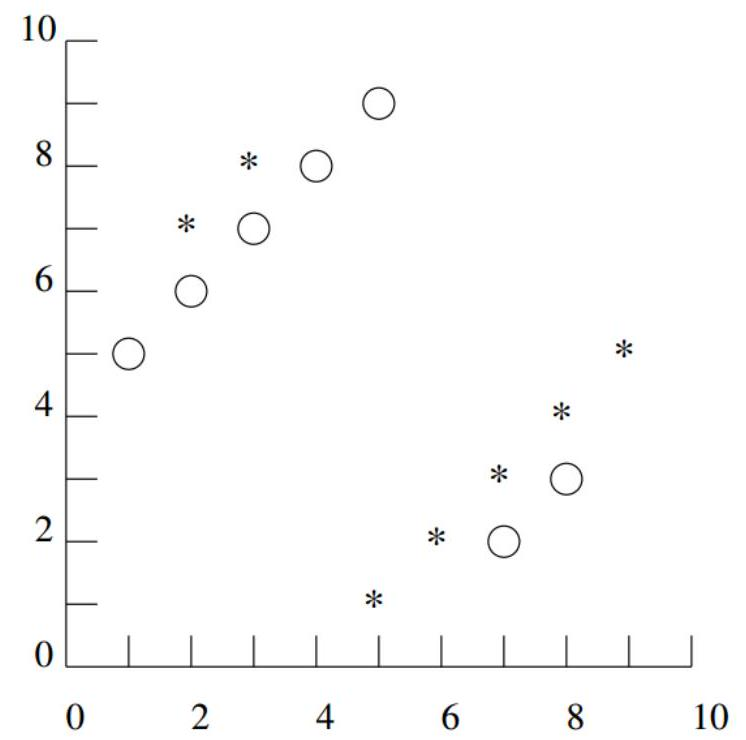
\includegraphics[max width=\textwidth]{2024_01_30_d638f3fd533378d9b317g-3}
\end{center}

(a) (3 pts) What value of $k$ minimizes training set error for this data set, and what is the resulting training set error? Why is training set error not a reasonable estimate of test set error, especially given this value of $k$ ?

\begin{flushleft}

\textbf{Answer 3a:} \\

- The training set error reaches its minimum at k = 1, leading to zero error. This outcome occurs as each data point's label is determined by its own label, given that the closest neighbor in this context is the data point itself. However, this approach does not serve as a reliable predictor for the test set error. \\
- It essentially leads to overfitting, where the model, although accurate with the training data, might fail to perform adequately with new, unseen data. This is because the model, in this case, doesn't account for the surrounding neighbors of a data point. As a result, while a k value of 1 perfectly fits the training data, its ability to generalize to new data could be significantly compromised, potentially reducing the accuracy of predictions on the test set. \\

    
\end{flushleft}

(b) (3 pts) What value of $k$ minimizes the leave-one-out cross-validation error for this data set, and what is the resulting error? Why is cross-validation a better measure of test set performance?

\begin{flushleft}

\textbf{Answer 3b:} \\
- Employing k values of either 5 or 7 yields the lowest error in Leave-One-Out Cross-Validation (LOOCV), with each leading to 4 instances of misclassification and 10 instances of correct classification. This gives us an error rate of 4/14. \\

- Cross-validation stands as a more robust indicator of a model's performance on unseen data compared to other methods. This is because it systematically alternates between different subsets of data for training and testing, ensuring that every data point gets a turn to be part of the test set. This process mitigates the likelihood of biases that might arise if a model is trained and evaluated on the same subset of data. Effectively, it offers a more comprehensive assessment by ensuring the model's performance is tested across the entire dataset. \\
    
\end{flushleft}

(c) (4 pts) What are the LOOCV errors for the lowest and highest $k$ for this data set? Why might using too large or too small a value of $k$ be bad?

\begin{flushleft}

\textbf{Answer 3c:} \\

Setting k to 0 yields an error rate of 0. Choosing k as 1 results in an error rate of 10/14. Opting for k equal to 13, on the other hand, produces an error rate of 14/14. Selecting excessively small or large values for k adversely affects the accuracy on the test set. Specifically, smaller values of k can lead to a model that overfits the training data, while larger values might result in underfitting, essentially reducing the problem to a basic majority voting system. This can lead to scenarios where all data points are misclassified, as seen in the given example.
    
\end{flushleft}

\hspace{1 cm}

\section*{4 Programming exercise : Applying decision trees and k-nearest neighbors $[50 \mathrm{pts}]$}
To work on this HW: you need to download two files (i) \href{http://nutil.py}{nutil.py} (ii) adult\_subsample.csv from here. Then copy/upload them to you own Google drive. If you cannot open the notebook with Colab or don't see an option, click on "Open with" and select "Connect more apps", where you can add Colab.

Next, for all the coding, please refer to the following colab notebook CS146-Winter2024-PS1.ipynb.

Before executing or writing down any code, please make a copy of the notebook and save it to your own google drive by clicking the File $\rightarrow$ Save a copy in Drive

\begin{center}
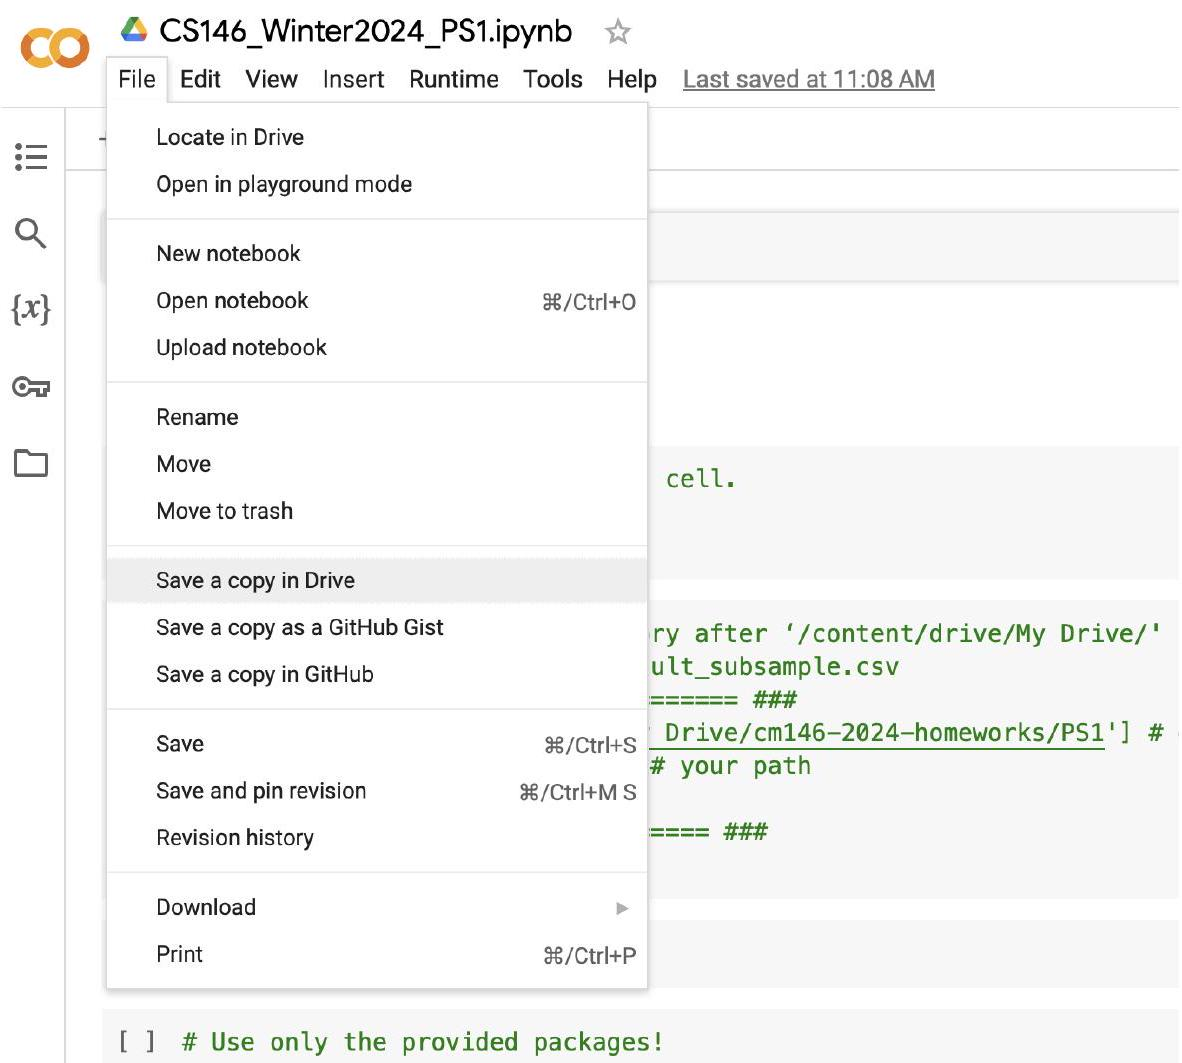
\includegraphics[max width=\textwidth]{2024_01_30_d638f3fd533378d9b317g-4(2)}
\end{center}

You will then be prompted to log into your google account. Please make sure all the work you implement is done on your own saved copy. You won't to able to make changes on the the original notebook shared for the entire class. Running the first two cells will further mount your own google drive so that your copy of the Colab notebook will have access to the two files (\href{http://nutil.py}{nutil.py} and adult\_subsample.csv) you have just uploaded.

The notebook has marked blocks where you need to code.

\begin{center}
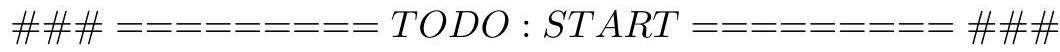
\includegraphics[max width=\textwidth]{2024_01_30_d638f3fd533378d9b317g-4(1)}
\end{center}

\begin{center}
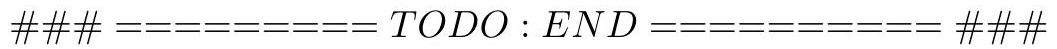
\includegraphics[max width=\textwidth]{2024_01_30_d638f3fd533378d9b317g-4}
\end{center}

For the questions please read below.

\subsection*{4.1 Visualization [5 pts]}
One of the first things to do before trying any formal machine learning technique is to dive into the data. This can include looking for funny values in the data, looking for outliers, looking at the range of feature values, what features seem important, etc.

Note: We have already converted all the categorical features to numerical ones. The target column is the last one: " $>50 \mathrm{k}$ ", where 1 and 0 indicate $>50 \mathrm{k}$ or $\leq 50 \mathrm{k}$ respectively. The feature "fnlwgt" describes the number of people the census believes the entry represents. All the other feature names should be self-explanatory. If you want to learn more about this data please click here

(a) (5 pts) Make histograms for each feature, separating the examples by class by running the function plot\_histograms in the notebook. This should produce fourteen plots, one for each feature, and each plot should have two overlapping histograms, with the color of the histogram indicating the class. For each feature, what trends do you observe in the data if any? (Please only describe the general trend. No need for more than two sentences per feature)

\begin{flushleft}

\textbf{Answer 4a:}\\

From the coding, I obtained these results:\\

\begin{figure}[H]
\centering
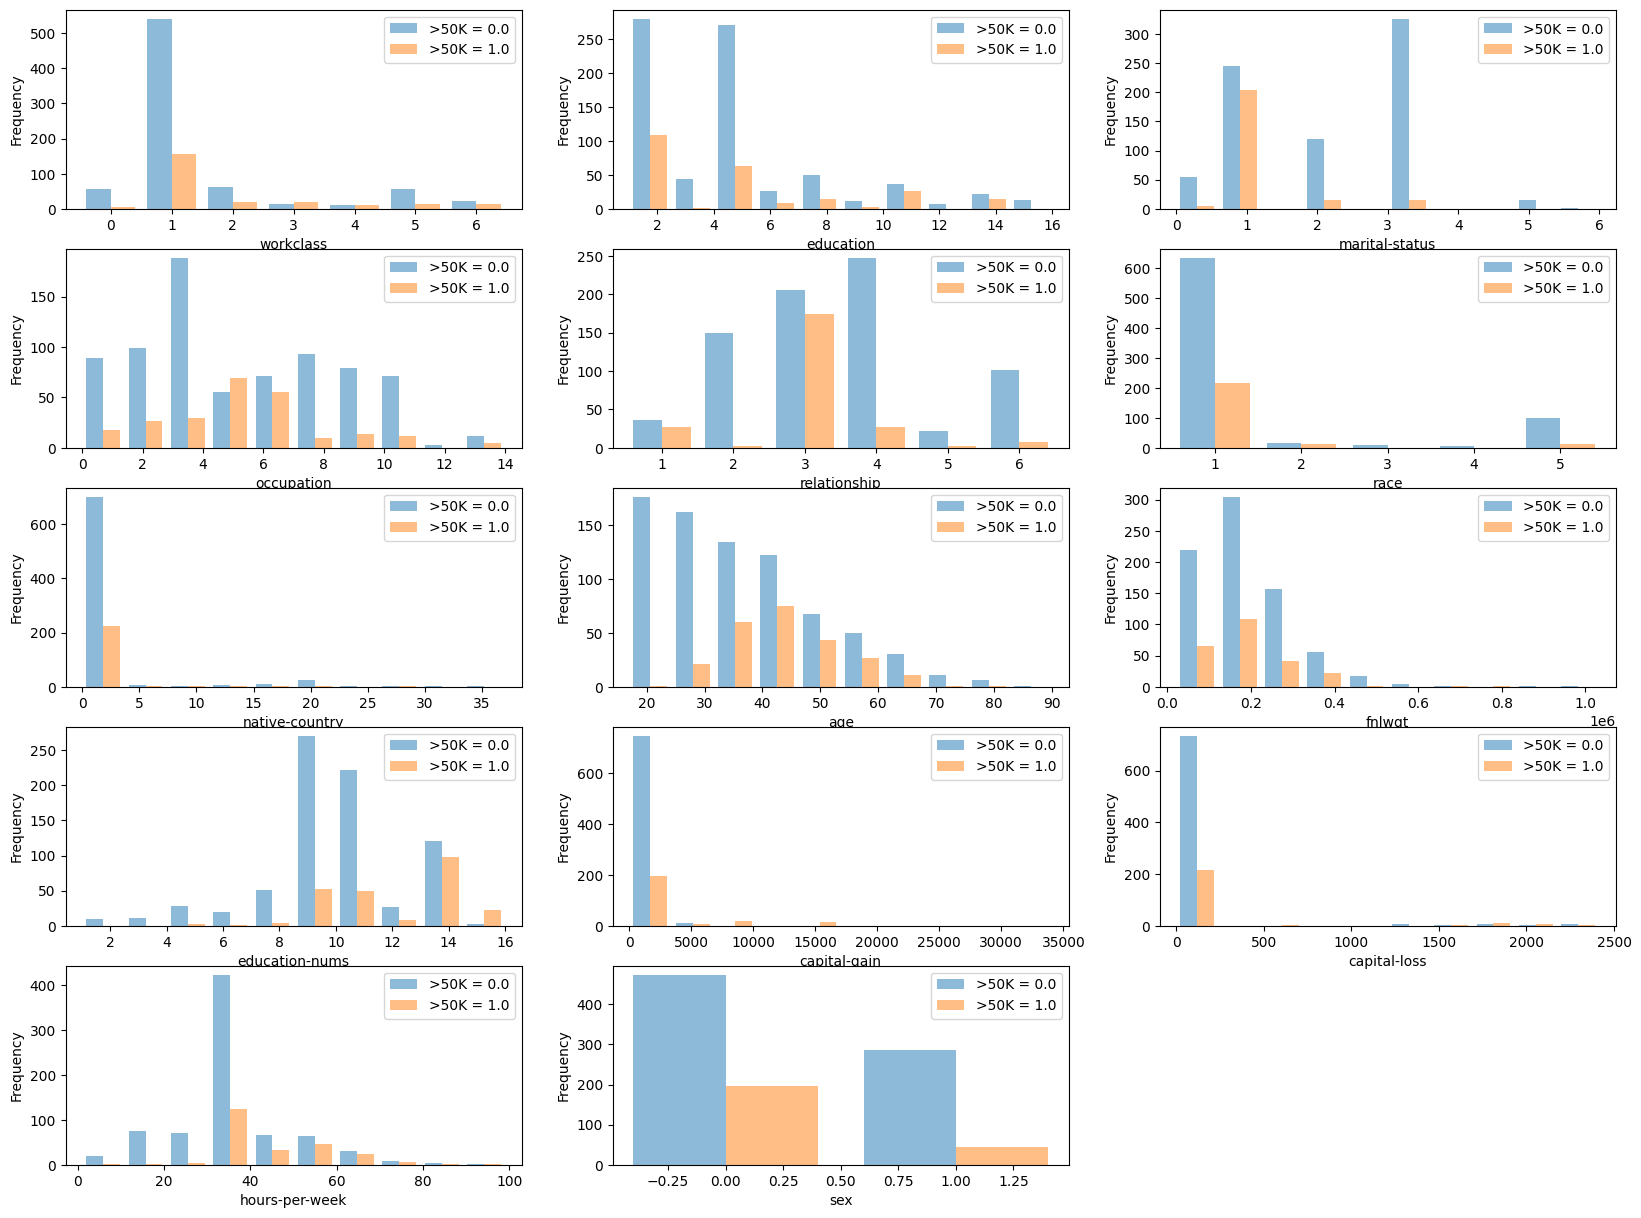
\includegraphics[width=1\textwidth]{histogram.png}
\caption{Histogram Results}
\label{fig:Histogram}
\end{figure}

\hspace{1 cm}

\begin{itemize}
  \item \textbf{Work Class:} A significant number of individuals are entrepreneurs, and among these, government employees are often found in the higher earning bracket of over \$50k.
  \item \textbf{Educational Attainment:} A higher education level frequently correlates with an increased likelihood of surpassing the \$50k annual earning mark.
  \item \textbf{Marital Status:} Divorced individuals have been observed to be more likely to earn above \$50k compared to their counterparts.
  \item \textbf{Type of Profession:} Careers in sales and executive management tend to be associated with incomes exceeding the \$50k threshold.
  \item \textbf{Relationship Status:} Being a husband is commonly linked to a greater chance of earning more than \$50k.
  \item \textbf{Ethnicity:} The dataset predominantly consists of white individuals, yet a notably large fraction of Asians are represented among those earning over \$50k.
  \item \textbf{Country of Origin:} Participants from the United States constitute the majority of the study's population, with most earning below \$50k.
  \item \textbf{Age Demographics:} The age group spanning from 40 to 50 years shows a higher propensity for incomes greater than \$50k.
  \item \textbf{Final Weight (Fnlwgt):} While the percentage of those earning more than \$50k does not vary widely, there exists a larger segment earning less than \$50k.
  \item \textbf{Educational Years (Education Nums):} Individuals with 8 to 10 years of education are most common, yet those with more than 14 years of education have a heightened chance of earning over \$50k.
  \item \textbf{Capital Gains:} Individuals with higher capital gains typically fall into the higher earning category of more than \$50k, despite most people reporting lower capital gains.
  \item \textbf{Capital Losses:} The majority experience lower capital losses, with those facing higher capital losses distributed evenly among income levels above and below the \$50k mark.
  \item \textbf{Weekly Working Hours:} A standard workweek hovers around 40 hours, yet it is observed that working more can correlate with earning more than \$50k.
  \item \textbf{Gender:} Despite a higher number of female participants in the study, they exhibit a relatively high likelihood of being in the over \$50k earning bracket.
\end{itemize}


\end{flushleft}

\subsection*{4.2 Evaluation $[45 \mathrm{pts}]$}

Now, let's use scikit-learn to train a DecisionTreeClassifier and KNeighborsClassifier on the data.

Using the predictive capabilities of the scikit-learn package is very simple. In fact, it can be carried out in three simple steps: initializing the model, fitting it to the training data, and predicting new values. ${ }^{1}$

(b) (0 pts) Before trying out any classifier, it is often useful to establish a baseline. We have implemented one simple baseline classifier, MajorityVoteClassifier, that always predicts the majority class from the training set. Read through the MajorityVoteClassifier and its usage and make sure you understand how it works.

Your goal is to implement and evaluate another baseline classifier, RandomClassifier, that predicts a target class according to the distribution of classes in the training data set. For example, if $85 \%$ of the examples in the training set have $>50 \mathrm{k}=0$ and $15 \%$ have $>50 \mathrm{k}=1$, then, when applied to a test set, RandomClassifier should randomly predict $85 \%$ of the examples as $>50 \mathrm{k}=0$ and $15 \%$ as $>50 \mathrm{k}=1$.

Implement the missing portions of RandomClassifier according to the provided specifications. Then train your RandomClassifier on the entire training data set, and evaluate its training error. If you implemented everything correctly, you should have an error of 0.374 or 0.385 .

\hspace{1 cm}

\begin{flushleft}

\textbf{Answer 4b:} \\
Classifying using Random... \\
	--training error: 0.374 \\

    
\end{flushleft}

(c) (10 pts) Now that we have a baseline, train and evaluate a DecisionTreeClassifier (using the class from scikit-learn and referring to the documentation as needed). Make sure you initialize your classifier with the appropriate parameters; in particular, use the 'entropy' criterion discussed in class. What is the training error of this classifier?

\hspace{1 cm}

\begin{flushleft}

\textbf{Answer 4c:} \\
Classifying using Decision Tree... \\
	--training error: 0.0 \\
    
\end{flushleft}

(d) (5 pts) Similar to the previous question, train and evaluate a KNeighborsClassifier (using the class from scikit-learn and referring to the documentation as needed). Use $k=3,5$ and 7 as the number of neighbors and report the training error of this classifier.

\hspace{1 cm}

\begin{flushleft}

\textbf{Answer 4d:} \\
Classifying using k-Nearest Neighbors... \\
	--training error k = 3 : 0.11399999999999999 \\ 
	--training error k = 5 : 0.129 \\
	--training error k = 7 : 0.15200000000000002 \\
    
\end{flushleft}

(e) (10 pts) So far, we have looked only at training error, but as we learned in class, training error is a poor metric for evaluating classifiers. Let's use cross-validation instead.


Implement the missing portions of error ( . . ) according to the provided specifications. You may find it helpful to use StratifiedShuffleSplit(...) from scikit-learn. To ensure that we always get the same splits across different runs (and thus can compare the classifier results), set the random\_state parameter to be the same (e.g., 0 ).

Next, use your $\operatorname{error}(\ldots)$ function to evaluate the average cross-validation training error, test error and test micro averaged F1 Score (If you dont know what is F1, please click here) of each of your four models (for the KNeighborsClassifier, use $k=5$ ). To do this, generate a random $80 / 20$ split of the training data, train each model on the $80 \%$ fraction, evaluate the error on either the $80 \%$ or the $20 \%$ fraction, and repeat this 100 times to get an average result.
\footnotetext{${ }^{1}$ Note that almost all of the model techniques in scikit-learn share a few common named functions, once they are initialized. You can always find out more about them in the documentation for each model. These are some-model-name.fit(...), some-model-name.predict(...), and some-model-name.score(...).
}

What are the average training and test error of each of your classifiers on the adult\_subsample data set?

\hspace{1 cm}

\begin{flushleft}

\textbf{Answer 4e:} \\
Investigating various classifiers... \\
Majority:	 train error =	 0.2399999999999996 \\
Majority:	 test error =	 0.2399999999999996 \\
Majority:	 F1 score =	 0.7600000000000002 \\
Random:		 train error =	 0.37477500000000014 \\
Random:		 test error =	 0.38199999999999984 \\
Random:		 F1 score =	 0.6180000000000002 \\
Decision Tree:	 train error =	 0.0 \\
Decision Tree:	 test error =	 0.20475 \\
Decision Tree:	 F1 score =	 0.7952500000000002 \\
KNN:		 train error =	 0.20167499999999997 \\
KNN:		 test error =	 0.25915000000000005 \\
KNN:		 F1 score =	 0.7408499999999998 \\

    
\end{flushleft}

(f) (5 pts) One way to find out the best value of $k$ for KNeighborsClassifier is $n$-fold cross validation. Find out the best value of $k$ using 10 -fold cross validation. You may find the cross\_val\_score (...) from scikit-learn helpful. Run 10-fold cross validation for all odd numbers ranging from 1 to 50 as the number of neighbors. Then plot the validation error against the number of neighbors, $k$. Include this plot in your writeup, and provide a 1-2 sentence description of your observations. What is the best value of $k$ ?

\hspace{1 cm}

\begin{flushleft}

\textbf{Answer 4f:} \\

\begin{figure}[H]
\centering
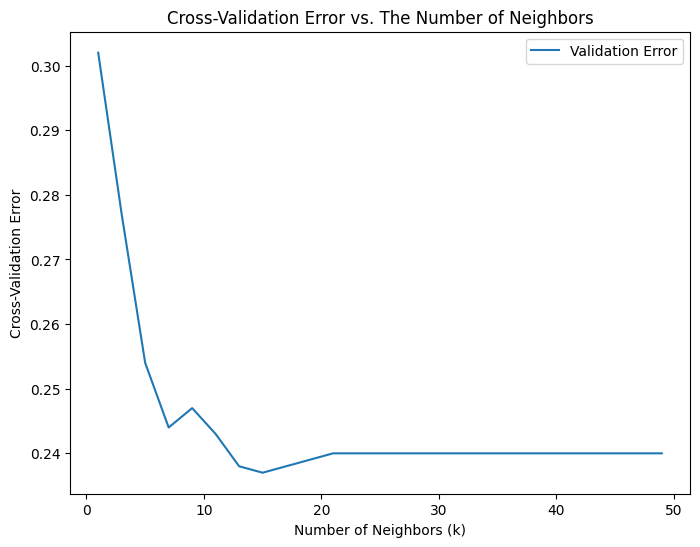
\includegraphics[width=1\textwidth]{images/error_vs_neighbor.png}
\caption{Validation Error vs Number of Neighbors}
\label{fig:Error}
\end{figure}

Finding the best k… \\
The best k value is: 15 with a validation error of: 0.2370000000000001 \\

    
\end{flushleft}

(g) (5 pts) One problem with decision trees is that they can overfit to training data, yielding complex classifiers that do not generalize well to new data. Let's see whether this is the case.

One way to prevent decision trees from overfitting is to limit their depth. Repeat your crossvalidation experiments but for increasing depth limits, specifically, $1,2, \ldots, 20$. You may find cross\_validate(...) from scikit-learn helpful. Then plot the average training error and test error against the depth limit. Include this plot in your writeup, making sure to label all axes and include a legend for your classifiers. What is the best depth limit to use for this data? Do you see overfitting? Justify your answers using the plot.

\hspace{1 cm}

\begin{flushleft}

\textbf{Answer 4g:}

\begin{figure}[H]
\centering
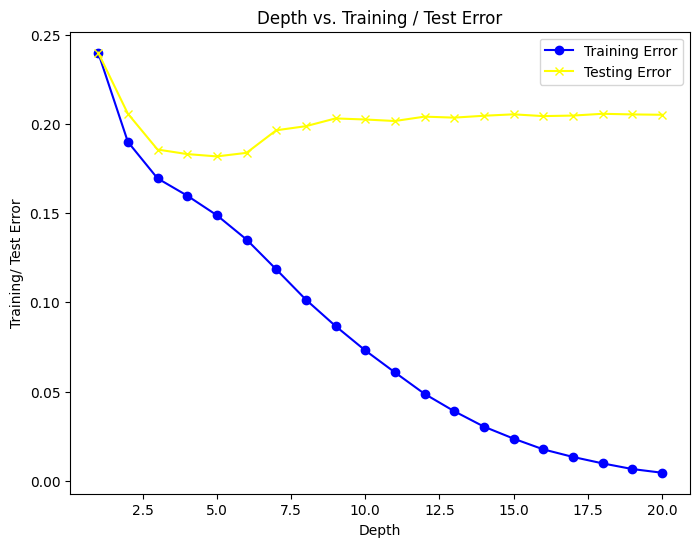
\includegraphics[width=1\textwidth]{images/depth_vs_error.png}
\caption{Depth vs Error (Go Warriors!)}
\label{fig:Depth}
\end{figure}

The best tree depth is: 5 with a validation error of: 0.17200000000000004
    
\end{flushleft}

(h) (5 pts) Another useful tool for evaluating classifiers is learning curves, which show how classifier performance (e.g. error) relates to experience (e.g. amount of training data). For this experiment, first generate a random 90/10 split of the training data using train\_test\_split from scikit-learn with random\_state set to 0 . Then, do the following experiments considering the $90 \%$ fraction as training and $10 \%$ for testing.

Run experiments for the decision tree and k-nearest neighbors classifier with the best depth limit and $k$ value you found above. This time, vary the amount of training data by starting with splits of 0.10 ( $10 \%$ of the data from $90 \%$ fraction) and working up to full size 1.00 ( $100 \%$ of the data from $90 \%$ fraction) in increments of 0.10 . Then plot the decision tree and $\mathrm{k}$-nearest neighbors training and test error against the amount of training data. Include this plot in your writeup, and provide a 1-2 sentence description of your observations.

\hspace{1 cm}

\begin{flushleft}

\textbf{Answer 4h:}

\begin{figure}[H]
\centering
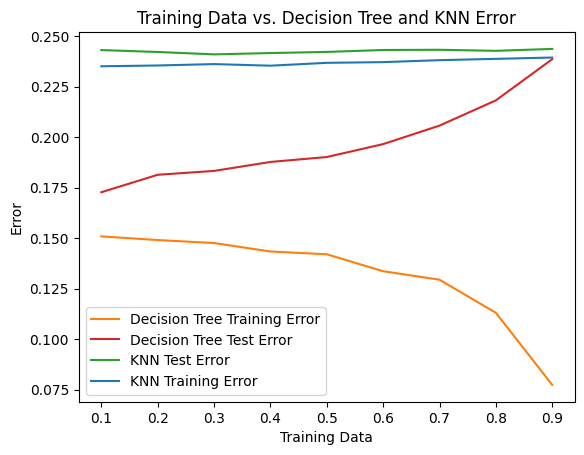
\includegraphics[width=1\textwidth]{images/training_error_vs.png}
\caption{Training vs Error}
\label{fig:Training}
\end{figure}

The Decision Tree's error is increasing with the amount of training data. This pitfall means that the training error is always less than the testing error.
    
\end{flushleft}

(i) (5 pts) Pre-process the data by standardizing it. See the sklearn.preprocessing.StandardScaler package for details. After performing the standardization such as normalization please run all previous steps part (b) to part (h) and report what difference you see in performance.

\hspace{1 cm}

\begin{flushleft}

\textbf{Answer 4i:}

\begin{figure}[H]
\centering
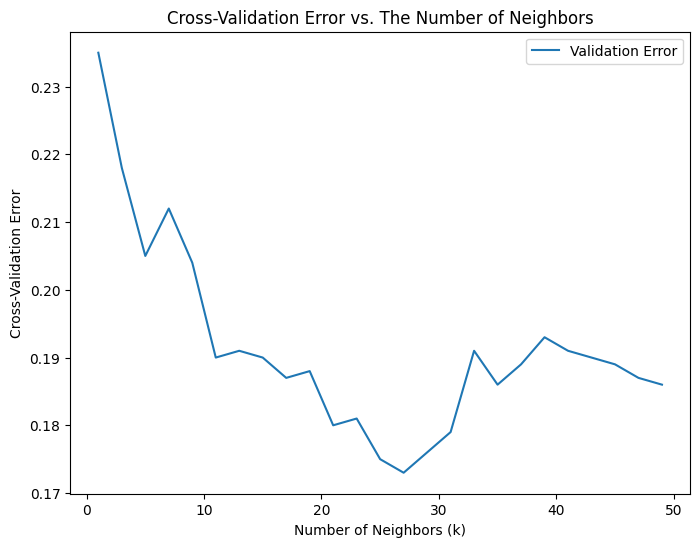
\includegraphics[width=1\textwidth]{images/val_error_vs_neighbors.png}
\caption{Validation Error vs Neighbors (Standard Scalar)}
\label{fig:Training}
\end{figure}

\begin{figure}[H]
\centering
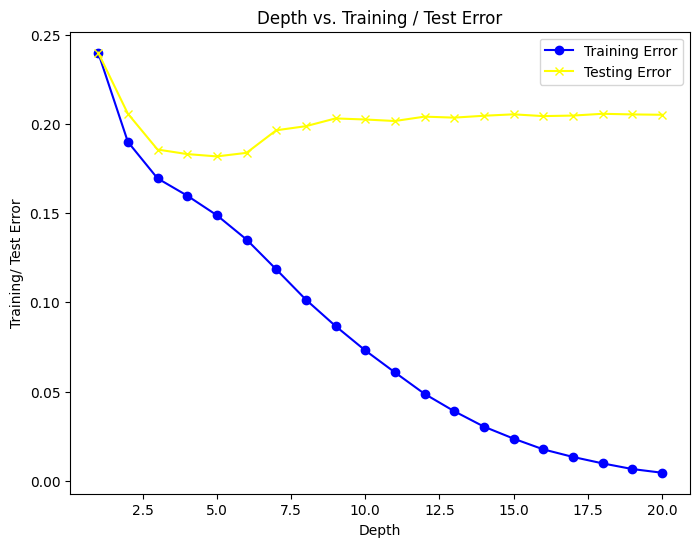
\includegraphics[width=1\textwidth]{images/depth_vs_error.png}
\caption{Depth vs Error}
\label{fig:Training}
\end{figure}

\begin{figure}[H]
\centering
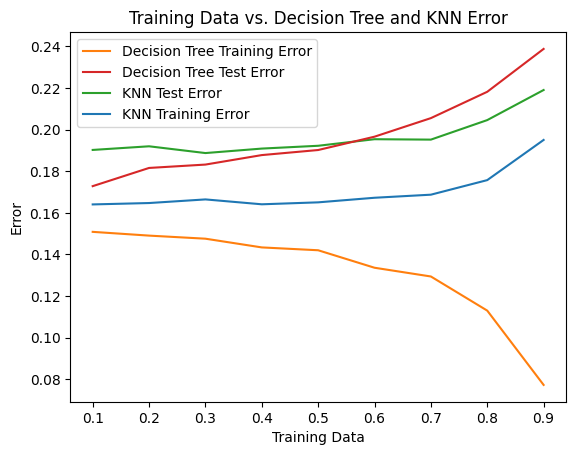
\includegraphics[width=1\textwidth]{images/train_data_vs_tree&knn.png}
\caption{Training Data vs Error Plot}
\label{fig:Training}
\end{figure}


Classifying using Majority Vote... \\
	-- training error: 0.240 \\
Classifying using Random... \\
	--training error: 0.374 \\
Classifying using Decision Tree... \\
	--training error: 0.0 \\
Classifying using k-Nearest Neighbors... \\
	--training error k = 3 : 0.11399999999999999 \\
	--training error k = 5 : 0.129 \\
	--training error k = 7 : 0.15200000000000002 \\
 \\

Investigating various classifiers... \\
Majority:	 train error =	 0.2399999999999996 \\
Majority:	 test error =	 0.2399999999999996 \\
Majority:	 F1 score =	 0.7600000000000002 \\
Random:		 train error =	 0.37477500000000014 \\
Random:		 test error =	 0.38199999999999984 \\
Random:		 F1 score =	 0.6180000000000002 \\
Decision Tree:	 train error =	 0.0 \\
Decision Tree:	 test error =	 0.20519999999999994 \\
Decision Tree:	 F1 score =	 0.7947999999999996 \\ 
KNN:		 train error =	 0.13265000000000002 \\ 
KNN:		 test error =	 0.20900000000000005 \\ 
KNN:		 F1 score =	 0.7910000000000004 \\

The best k value is: 27 with a validation error of: 0.17300000000000004 \\

\hspace{1 cm}

Observations: \\
For Random Classifier, Decision Trees, and Majority: there was no differnece. \\
However, for KNN, there was a indeed a noticeable increase. Also the best k value increase to 27 from the 15. \\

\end{flushleft}


\end{document}